
\chapter{Experiments}
\label{chap:Experiments} 

The success of the reconstruction largely depends on the representation of the data
after the feature-map is applied.
Relying on the mean and variance of the data to accurately describe the data distribution 
relies on a strong assumption.
More sophisticated ways of capturing data distributions exist, yet mean and variance were chosen due to their simplicity in evaluation and computation of the gradients.

The feature-map ideally "disentangles" the data space to enable 
these simple statistics to capture enough of the complexity of the data set.

In order to assess the efficacy of the neural network's latent representations 
and their ability to capture the data distribution by these statistics,
several different mappings or methods will be compared. 

First, in order to establish the notation used throughout, in \cref{sec:nn_def}, 
a short introduction on the multi-layer perceptron (MLP) is given,
Then, the various feature-mappings or methods will be presented in \cref{sec:methods}.
Following that, the three data sets used in the experiments are introduced in \cref{sec:datasets},
and finally, the perturbation and reconstruction models are depicted in \cref{sec:reconstruction_models}.
\Cref{sec:evaluation} deals with evaluation metrics.

\section{Neural Network}
\label{sec:nn_def}

In a classification setting, a \textbf{neural network} $\Phi$ is a function that maps an input $\vec x \in \R^d$ to an output $\in \R^C$,
often referred to as the unnormalized logits. 
The network makes its prediction by returning the index of the maximal value of the logits.
The classic neural network is a \textbf{multi-layer perceptron} (MLP) or fully-connected (FC) neural network.
Here, every input of a layer is connected to every output of the layer.
Every node of any layer receives its input as a weighted sum over all of the previous layer's activations.
This weighted sum is passed through a non-linear activation function, often one of either the rectified-linear unit (ReLU) or sigmoid, to form the node's activation. 
This is done for all nodes in a layer before being passed on to the next.
A full network thus is a composition of functions $\Phi_\ell$, or \textbf{layers} that 
successively act on the outputs $\vec h$ of the previous layer, called \textbf{activations} or \textbf{hidden states}. 
In a plain \textbf{fully-connected} neural network, the layers are each made up of an affine linear transformation and a non-linear activation function.

Formally, a fully-connected neural network of layer depth L is described as:

\[
    \Phi : \R^d \to \R^C
\]
\[
    \Phi = \Phi_\text{L} \circ \ldots \circ \Phi_1
\]
\[
    \vec h_\ell = (\Phi_\ell \circ \ldots \circ \Phi_1) (\vec x) =
    \Phi_\ell(\vec h_{\ell-1}) \in \R^{d_\ell}
\]
$\Phi_\ell$ then, is a mapping from $\R^{d_{\ell-1}}$ to $\R^{d_\ell}$ and $\R^{d_\textnormal{L}} = \R^C$.
% The space of a hidden state $\vec h$ is called a \textbf{feature-space}.
The input $\vec x$ is sometimes also referred to as $\vec h_0$ and $\R^{d_0} := \R^d$.
The layers themselves contain as parameters a \textbf{weight matrix} $\vec W$ and a \textbf{bias} $\vec b$
that together form an affine linear transformation.
\[
    \Phi_\ell(\vec h) = \sigma (\vec W \vec h + \vec b) \comma{where}
    \vec W \in \R^{d_\ell \times d_{\ell-1}} \text{ and } 
    \vec b \in \R^{d_\ell}
\]

The non-linear activation function $\sigma$ is often a function $\sigma:\R\to\R$ that is applied element-wise.



\section{Methods}
\label{sec:methods}

The following methods introduce various feature-mappings.
Each feature-mapping $\varphi$ induces a loss function $\loss_\varphi$ as outlined in \cref{eqn:statistics_loss}.
For every method there exists a class-dependent loss formulation $\loss_\varphi^{\mathcal C}$,
as given in \cref{eqn:class_statistics_loss}.
The abbreviations to the methods are given in parenthesis in the following headers. 
When referring to the class-dependent formulation CC (class-conditional or
class-constrained) is added to the abbreviation.

The complete loss formulation that is used in the optimization process 
for a given feature-map $\varphi$, a target data set $\set A$ and a source data set $\set B$ 
is a composite loss given by
\[
    r_\text{stats}\loss_\varphi(\set A, \set B) + r_\text{crit}\loss_\text{crit}(\set B, y_{\set B}) \,,
\]
where $y_{\set B}$ are the target labels and $\loss_\text{crit}$ is the criterion loss, which, throughout this work, is the cross-entropy loss.
It is the loss function that was used for optimizing the parameters of the neural network.



\subsection{Neural Network - Second-to-Last Layer (NN)}

Given a neural network $\Phi$ of depth L,
a feature-mapping can be obtained by mapping inputs to the second-to-last layer $\Phi_{\text{L}-1}$, 
the layer before the logits layer.
\[
    \varphi : \R^d \to \R^{d_\textnormal{L-1}} = (\Phi_\textnormal{L-1} \circ \dots \circ \Phi_1)
\]
Generally, this layer is considered to encode a highly abstracted representation of the data
and typically contains the signal in a comparatively high dimensional space, before it's
reduction to a $C$-dimensional vector by the logits-layer.
% which contains the least amount of information  on the input.
In convolutional neural networks, where one often deals with images
of a specified input shape (the Cartesian product of channels$\times$height$\times$width), 
the spatial relationship of features is kept throughout the forward propagation by the layers.
In this layer, the entire signal is flattened down to a single $d^{\text{L}-1}$-dimensional vector, 
before being passed to the logits-layer.
As an activation function is normally not needed on the last layer when returning the index of the maximal value, 
the logits-layer has to be able to linearly classify its input - the last hidden state - in order to 
give the final prediction.
This warrants the belief that this layer contains the most disentangled representation of the data.


\subsection{Neural Network - All Layers (NN ALL)}

All hidden states together of the neural network can be seen as outputs of a collection of feature-maps [$\varphi_0, \dots, \varphi_\text{L}$], where
\begin{alignat*}{2}
    \varphi_\ell &: \R^d \to \R^{d_\ell} &&= (\Phi_\ell \circ \dots \Phi_1)
    \comma{for $\ell = 1, \dots$, L - 1}  \,, \\
    \varphi_\textnormal{L} &: \R^d \to \R^d &&= \Id \,.
\end{alignat*}





\subsection{Random Projections (RP)}
To contrast the efficacy of the previous two feature-representations on the success of the optimization process,
a feature-mapping involving one linear layer is used. This is done by selecting a number of  random linear projections.
A random projection is a linear mapping $r: \R^d \to \R$.
It is created by choosing a normalized random vector $\vec v \in S^{d-1} = \{\vec x \in \R^d : \|\vec x\| = 1\}$.
It can be seen as a linear projection to the one-dimensional subspace defined by the vector $\vec v \in \R^d$.
\[
    r(\vec x) = \vec v ^\top \vec x
\]
By choosing a total of $s_\text{RP}$ random vectors $\{v_1, \dots, v_{s_\text{RP}}\}$ one obtains a linear mapping $R: \R^d \to \R^n$:
\[
    R(\vec x) = \vec V \vec x =
    \begin{bmatrix}
        - \vec v_1 ^\top - \\
        \vdots \\
        - \vec v_n ^\top - \\
    \end{bmatrix}
    \vec x =
    \begin{bmatrix}
        \vec v_1 ^\top \vec x \\
        \vdots \\
        \vec v_n ^\top \vec x \\
    \end{bmatrix}
\]
%
% The loss function $\loss_R$ stays as was defined before.
In order to obtain a more balanced output,
the projection can be centered around an origin $\vec o$.
% 
\[
    R_{\vec o} (\vec x) = \vec V (\vec x - \vec o) \,,
\]
where $\vec o \in \R^d$ is the new origin of the projection. 
The idea is to set the origin to be center of the target data set $\set A$. $\vec o = \mean (\set A)$
This way, the data after the projection will be centered around $\vec 0$.
In practical applications, the data often is normalized and $\vec 0$-centered beforehand,
yet the class-dependent variant can be modified to select an origin $\vec o_c$ for each class $c$.
\cref{eqn:class_statistics_loss} then becomes:
% 
\begin{equation*}
    \loss _{\text{RP}} ^{\mathcal C} (\set A, \set B) =
    \sum _{c = 1, \dots, C}
    \begin{alignedat}[t]{1}
        \|\mean ({R_{\vec o_c} (\set A|_c)}) - \mean ({R_{\vec o_c} (\set B|_c)}) &\| \\
        {} + \|\var ({R_{\vec o_c} (\set A|_c)}) - \var ({R_{\vec o_c} (\set B|_c)}) &\|  \,,
    \end{alignedat}
\end{equation*}
% \begin{align}
% \begin{split}
% \label{eqn:class_statistics_loss}
%     \loss _\varphi ^\text{CC} (\set A, \set B) =
%     \sum _{c = 1, \dots, C}
%     \|\mean ({R_{\vec o_c} (\set A|_c)}) - \mean ({R_{\vec o_c} (\set B|_c)}) &\| \\
%     {} + \|\var ({R_{\vec o_c} (\set A|_c)}) - \var ({R_{\vec o_c} (\set B|_c)}) &\|  \,,
% \end{split}
% \end{align}
%
where $\vec o_c$ is set to the mean of each class $\mean ({\set A|_c})$.


\subsection{Random projections ReLU (RP ReLU)}
To further explore the importance of the non-linear activation functions contained within the network,
the previous method is modified by applying an activation function, in this case the ReLU to the output.
% 
\[
    R_{\vec o}^+ (\vec x) = (\vec V (\vec x - \vec o))^+ \,,
\]
where $(\,\cdot\,)^+ :\R^n \to \R^n$ is the projection onto the positive orthant. It applies $\max(0, \cdot)$ element-wise.

Since the layers of a neural network that use ReLU activation functions have a bias parameter that shifts the threshold above which an input can pass unaltered, this will also be incorporated.
\[
    R_{\vec o}^{\vec b} (\vec x) = (\vec V (\vec x - \vec o) + \vec b)^+ \,,
\]
where $\vec b \in \R^d$ is the bias. For a target dataset $\set A$, it is chosen as $\vec b \sim \mathcal N(\vec 0, \textnormal{diag}(\boldsymbol \sigma ^2))$, 
where $\boldsymbol \sigma ^2 = \var ({R_{\vec o}(\set A)})$.

The class-dependent variant can again make use of more suited biases $\vec b_c \sim \mathcal N( \vec 0, \textnormal{diag}(\boldsymbol \sigma _c^2))$, 
where $\boldsymbol \sigma_c ^2 = \var ({R_{\vec o_c}(\set A|_c)})$.
In this case, \cref{eqn:class_statistics_loss} becomes:
% 
\begin{equation*}
    \loss _{R^+} ^\text{CC} (\set A, \set B) =
    \sum _{c = 1 \dots C}
    \begin{alignedat}[t]{1}
        \|\mean ({R_{\vec o_c}^{\vec b_c} (\set A|_c)}) - \mean ({R_{\vec o_c}^{\vec b_c} (\set B|_c)}) &\| \\
        {} + \|\var ({R_{\vec o_c}^{\vec b_c} (\set A|_c)}) - \var ({R_{\vec o_c}^{\vec b_c} (\set B|_c)}) &\| 
    \end{alignedat}
\end{equation*}

\subsection{Randomly Initialized Neural Network (RANDOM NN)}
To further study the importance of an optimized feature-representation of a trained neural network, 
the same neural network model with randomly initialized parameters is evaluated and compared.
This could give insight to the importance of the number of compositions of non-linear transformations.

\subsection{Combinations (COMBINED)}
All previously defined feature-maps can be combined into a new collection of feature-maps,
in order to obtain a new loss formulation.
One combination in particular, the mixture of all neural network layers (NN ALL) and random projections (RP) is further examined in the following experiments.


\section{Data Sets}
\label{sec:datasets}

\subsection{GMM}
\label{sec:datasetgmm}
A dataset made up of Gaussian mixture models (in the following \textit{GMM}), 
is made up of $C$ classes, each of which contains $n_\text{mode}$ clusters or modes of multivariate Gaussian normal distributions. The probability-density function (pdf) is as follows.
\begin{align}
\label{eqn:gmm_distr}
    p(\vec x) &= \frac 1 C \sum_{c=1}^C p(\, \vec x \mid c \,) \nonumber\\
    p(\, \vec x \mid c \,) &= \frac 1 {n_\text{mode}} \sum _{m=1}^{n_\text{mode}}
    \mathcal N (\gamma \vec m_c + \lambda \boldsymbol \mu_c^{(m)}, \boldsymbol \Sigma_c^{(m)}) \, ,
\end{align}
where \\
$\vec m_c \sim \mathcal N (\vec 0, \vec I)$ is the center for each class $c=1,\ldots, C$ ,\\
$\boldsymbol \mu_c^{(m)} \sim \mathcal N (\vec 0, \vec I)$ and
$\vec \Sigma_c^{(m)}$ are the center and the covariance matrix of the multivariate normal distribution
for each mode $m=1,\ldots, n_{\textnormal{mode}}$ and class $c=1,\ldots, C$.  \\
A positive semi-definite matrix $\vec \Sigma_c^{(m)}$ is generated by choosing $d$ eigenvalues $\vec e = (e_1, \ldots, e_d)$, $e_i \sim \mathcal U(\alpha, \beta)$, for all $i=1, \ldots, d$, for some $\alpha, \beta > 0$ and 
by sampling a random orthogonal matrix $\vec Q$. 
This can be done for example by choosing $\vec Q = \{q_{ij}\}_{i,j=0}^{d}$, 
where $q_{ij} \sim \mathcal N(0, 1)$
and creating an orthonormal basis via Gram-Schmidt. 
\begin{align*}
    \vec \Sigma_c^{(m)} = \vec Q^\top \text{diag}(\vec e) \vec Q
\end{align*}

\begin{figure}[h]
    \centering
    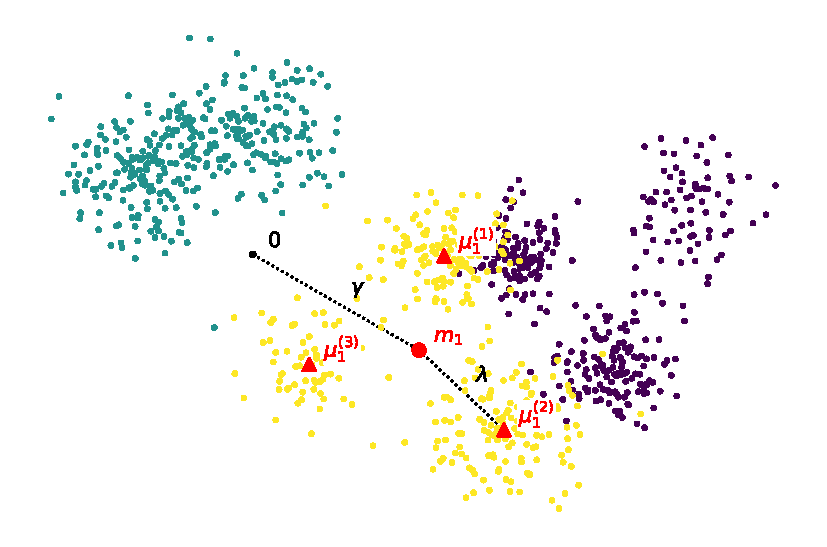
\includegraphics{figures/GMM_plot.pdf}
    \caption{GMM data set example for $d=2$, $C=3$, $n_\text{modes}=3$; 
    $\gamma$ and $\lambda$ control the standard-deviation of the distance of the class-center and the center of the modes respectively. $\alpha$ and $\beta$ control the size and orientation of the clusters}
    \label{fig:gmm_plot}
\end{figure}

For a given data set size, the labels are generated by equally sampling from all classes $1, \ldots, C$.
Then the input will be sampled according to the conditional probability-density function given by \cref{eqn:gmm_distr}.
The specific parameters used for generating the data set in all the experiments
are given in \cref{AppendixParameters}.


\subsection{MNIST}
MNIST, a common data set used in pattern recognition, is made up of 70000 black-and-white images 
of handwritten digits from 0 to 9. 
Each image is made up of 28$\times$28 pixels, totaling an input dimension of $d=784$.
\XXX{show example, give source}

\subsection{CIFAR-10}
CIFAR10 contains 60000 colored images from 10 non-overlapping categories or classes.
Each image has an input shape of $(3, 32, 32)$ as it comes with 3 color channels 
and has a dimension of 32$\times$32 pixels, resulting in a total of $d=3072$ dimensions.
\XXX{show example, give source}





\section{Perturbation and Reconstruction Models}
\label{sec:reconstruction_models}


\subsection{Gaussian Mixture Models}

The \textbf{perturbation} for the GMM data set is modeled by
a random affine-linear transformation.
The linear part consists of an identity transformation with added Gaussian noise
and the translation vector is also sampled by Gaussian noise.
The standard deviation of the noise is controlled by a parameter $\kappa > 0$.
\[
    \delta(\vec x) = (\vec I + \kappa \vec N)\vec x + \kappa \mu \,,
\]
where $\vec N = \{n_{i, j}\}_{i j = 1}^{d}$, $n_{ij} \sim \mathcal N (0, 1)$ for all $i, j = 1 , \ldots, d$
and 
$\mu = \{\mu_i\}_{i=0}^d$, $\mu_i \sim \mathcal N(0, 1)$ for all $i=1,\ldots,d$.
This transformation is in invertible if $\det (\vec I + \kappa \vec N) \neq 0$ with P=1,
\XXX{talk about invertibility?}
For $\kappa = 0$, the identity transformation is obtained.

The \textbf{reconstruction model} for this data set is also an affine-linear transformation. 
$\rho(\vec x) = \vec A \vec x + \vec b$.
$\vec A$ and $\vec b$ make up the model's learnable parameters, and
these are initialized to $\vec A = \vec I$ and $\vec b = \vec 0$ in order to form the identity transformation.
An optimal solution is given by
$\vec A^* = (\vec I + \kappa \vec N)^{-1}$, $\vec b^* = -\kappa \vec A^* \boldsymbol \mu$.
Proof:
\begin{equation}
\label{eqn:gmm_optimal}
\begin{split}
    \rho^* ( \delta (\vec x)) 
    &= \vec A^* ((\vec I + \kappa \vec N)\vec x + \kappa \boldsymbol \mu) + \vec b^* \\
    &= \vec A^* (\vec I + \kappa \vec N)\vec x + \kappa \vec A^* \boldsymbol \mu + \vec b^* \\
    &= \vec x
\end{split}
\end{equation}

\subsection{Image Data Sets}

\subsubsection{Perturbation Model}

The \textbf{perturbation model} for the image data sets MNIST and CIFAR10
is a composition of additive Gaussian noise and two noise-controlled 2d-convolutions.
\XXX{talk about 2d-convolutions?}

\[
    \delta(\vec x) = \vec K_2(\vec K_1(\vec x + \mu)
\]

The convolutions $\vec K_n$ are given by kernel matrices $\vec k_n$ of size $3\times3$ for $n=1,2$.
The kernel matrices are set to the identity kernel with added Gaussian noise, controlled by $\kappa$.
The identity kernel for the MNIST data set (which only contains one "color" channel) is given by 
% \eqnref{eqn:kernelid}.
\begin{equation*}
% \label{eqn:kernelid}
    \vec k_{\text{id}} = \begin{bmatrix}
        0 & 0 & 0 \\
        0 & 1 & 0 \\
        0 & 0 & 0 \\
    \end{bmatrix} \,.
\end{equation*}
For the CIFAR10 data set, where 3 color channels are present, the input shape is of (3, 32, 32). 
In order to obtain the same output shape, 
a total of $3*3=9$ convolution kernels $\vec k^{[i,j]}$ for $i,j=1,2,3$ are needed per convolution.
The output of channel $j$ is given by $\sum_{i=1}^{3} \vec x * \vec k^{[i, j]}$.
The identity convolution can be achieved by setting 
\[
    \vec k^{[i,j]} = \begin{cases}
        \vec k_{\text{id}} &, \text{ if } i = j\\
        \vec 0 &, \text{ otherwise} \\
    \end{cases} \,.
\]

This convolution operator is in general not invertible for $\kappa > 0$.
\XXX{Proof??}
Again, for $\kappa = 0$, the identity transformation is obtained.

For the output to contain the same dimensions as the input, the input needs to be \textit{padded}.
The 'reflection' padding was chosen.
\XXX{Should elaborate}


\subsubsection{Reconstruction Model}

\begin{figure}[!ht]
\begin{minipage}{0.5\textwidth}
\centering
\input{Figures/ChartInvertblock}
% \caption*{ResNet - Residual Layer}
\end{minipage}
\begin{minipage}{0.5\textwidth}
\centering
\begin{tikzpicture}[node distance=0.58cm and 1.7cm, auto]

\node [] (input) {Input};
\node [layer, below= 1cm of input, fill=Dandelion!9] (conv1) {Conv1x1};
\node [layer, below= of conv1] (res1) {Residual Layer};
\node [layer, below= of res1] (res2) {Residual Layer};
\node [below= of res2, minimum height=0.8cm] (res3) {\dots};
\node [layer, below= of res3] (res4) {Residual Layer};
% \node [layer, below= 1cm of input, fill=Dandelion!9] (conv1) {Conv3x3};
% \node [layer, below= of conv1, fill=Blue!5] (bn1) {BatchNorm};
% \node [layer, below= of bn1, fill=Mahogany!7] (relu) {ReLU};
% \node [layer, below= of relu, fill=Dandelion!9] (conv2) {Conv3x3};
% \node [layer, below= of conv2, fill=Blue!5] (bn2) {BatchNorm};
\node [below= 1cm of res4] (output) {Output};

% \path (input) -- node[anchor=center] (branch) {} (conv1);
% \path (bn2) -- node[circle, draw, minimum size=0.6cm, anchor=center] (plus) {} (output);
% \node at (plus) {+};

% \node [right= 1.6cm of branch] (dummy) {};
\node [draw, dashed, inner sep=0.25cm, fit=(res1)] {};

% \draw [larrow, rect connect v=2cm] (branch.center) to (plus.east);

\draw [larrow] (input) to (conv1);
\draw [larrow] (conv1) to (res1);
\draw [larrow] (res1) to (res2);
\draw [larrow] (res2) to (res3);
\draw [larrow] (res3) to (res4);
\draw [larrow] (res4) to (output);
% \draw [larrow] (bn1) to (relu);
% \draw [larrow] (relu) to (conv2);
% \draw [larrow] (conv2) to (bn2);
% \draw [larrow] (bn2) to (plus);
% \draw [larrow] (plus) to (output);


\end{tikzpicture}
% \caption*{ResNet - Residual Layer}
\end{minipage}
\caption{ResNet architecture}
\label{fig:resnet}
\XXX{add ReLU out + 1x1conv}
\end{figure}

The model for the reconstruction task on images is given by a residual network architecture
as outlined in \cref{fig:resnet}. 
The network \textit{width}, the number of individual convolutional kernels, is controlled by the parameter $s_\text{width}$; the \textit{depth}, the number of residual layers, by the parameter
$s_\text{depth}$.

The default parameters for the experiments are given in \cref{AppendixParameters}.




\section{Evaluation}
\label{sec:evaluation}

\begin{figure}[ht]
    \centering
    \begin{tikzpicture}[node distance=1cm and 1.7cm, auto]

\node (A) [node, fill=red!7] {\textbf{Target} \\ $\set A$};
\node (B) [node, below= of A] {\textbf{original} \\ $\set B_\text{true}$};
\node (C) [node, below= 2.2cm of B, fill=blue!0] {\textbf{Validation} \\ $\set C_{true}$};

\node (Bp) [node, right= of B, fill=blue!2] {perturbed \\ \textbf{Source} \\ $\set B$};
\node (Br) [node, right= of Bp, fill=blue!7] {\textbf{reconstructed} \\ $\rho^* (\set B)$};


\draw [arrow, dashed, thin] (B) -- (Bp) node (Pert) [midway, function, dashed] {$\delta$};
\draw [arrow] (Bp) -- (Br) node (Rec) [midway, function] {$\rho^*$};
\node [fill=white, below= 0cm of Pert] {\footnotesize \textit{unknown}};
\node [fill=white, below= 0cm of Rec] {\footnotesize \textit{learned}};


\node (Net) [function, fill=gray!5, above= of Br] {Neural \\ Network};
\node (vNet) [function, fill=gray!5, right= of Net] {verification \\ Neural \\ Network};

\draw [arrow, Mahogany, thin, bend left=20] (A) to (Net);
\draw [arrow, Mahogany, thin, bend left=20] (A) to node[below] {\footnotesize trained} (vNet);
\draw [arrow, Blue, thin] (Net.210) to[bend right=20] node [midway, above, sloped] {\footnotesize optimized} (Rec.north);

\node (Cp) [node, right= of C, fill=blue!0] {\textbf{perturbed} \\ $ {\set C}$};
\node (Cr) [node, right= of Cp, fill=blue!0] {\textbf{reconstructed} \\ $\rho ^*( {\set C})$};


\draw [arrow, dashed, thin] (C) -- (Cp);
\draw [arrow] (Cp) -- (Cr);

\draw [arrow, dashed, thin] (C) -- (Cp) node (Pert) [midway, function, dashed] {$\delta$};
\draw [arrow] (Cp) -- (Cr) node (Rec) [midway, function] {$\rho^*$};

\draw [arrow, <->, thin, OliveGreen] (Br.south) to [rect connect h=-0.75cm] (B.south);
\draw [arrow, <->, thin, OliveGreen] (Cr.north) to [rect connect h=0.75cm] (C.north);

\path (Br.east) to [out=0, in=270]  node [near end, OliveGreen, xshift=0.1cm] {accuracy} (vNet.265);
\draw [arrow, thin, OliveGreen] (Br.east) to [out=0, in=320] (Net.315);
\draw [arrow, thin, OliveGreen] (Cr.east) to [out=0, in=320] (Net.325);
\draw [arrow, thin, OliveGreen] (Cr.east) to [out=0, in=270] (vNet.south);


\node [OliveGreen] at ($(Bp)!0.5!(Cp)$) {IQA metrics};

\node [below= 1.5cm of Pert] (Id) {Id};
\path (Id) -| node[anchor=center] (Idr) {$\hat {\Id}$} (Rec);
\draw [arrow] (Id) -- 
node[near start, xshift=0.2cm, function] {$\delta$} 
node[near end, xshift=-0.2cm, function] {$\rho^*$} (Idr);
\draw [arrow, <->, thin, OliveGreen] (Idr.south) to [rect connect h=-0.6cm] (Id.south);
\node [OliveGreen, yshift=-1.2cm] at ($(Id)!0.5!(Idr)$) {rel. error};
% \node [circle, fill=blue] at (Idr){};
% \draw (0,0)|-node{mid}(2,3);
% \node [below= 1cm of Rec] {};
% \node (Cbelow) [below= of Cp] {EEE};
% \draw [arrow, dashed, thin] (C) -- (Cp) node (Pert) [midway, function, dashed] {$\delta$};
% \draw [arrow] (Cp) -- (Cr) node (Rec) [midway, function] {$\rho^*$};

\end{tikzpicture}
    \caption{Overview of evaluation metrics}
    \label{fig:evaluation_overview}
    \centering
\end{figure}

The result of the reconstruction task on the GMM data set can be evaluated by the \textbf{accuracy}
of the neural network. However, this however is likely to exhibit a strong bias in the classification accuracy 
towards the source data set $\set B$, as it, and 
the neural network 
are used in the optimization process
of many of the presented methods.
For this reason, the same transformations are applied to
a validation set $\set C$, and the 
correct classification rate will be reported as the \textbf{validation accuracy}. 
Because none of the data points in $\set C$
are used during optimization, it is, to some extent, a measure of generalization
of the learned transformation $\rho^*$.

A second measure of generalization can be made by evaluating the accuracy of an
independently trained neural network, the verification neural network.
The accuracy of the validation set $\set C$ on this second neural network 
constitutes the \textbf{verification accuracy}.

In the case of the GMM data set, since the explicit probability density function (pdf) is known, 
(see \ref{eqn:gmm_distr}), the estimated \textbf{cross-entropy}, given by
\begin{equation}
\label{eqn:cross_entropy}
    H(\set A) = - \frac 1 {|\set A|} \sum_{i=1}^{|\set A|} \log p(\vec x_i)
\end{equation}
is used as a measure of unlikelihood of $\set A$ coming from the underlying distribution.

% For the main reconstruction task, 
% five metrics will be studied to determine a methods success (along with visual appeal).
% For one, the accuracy of the reconstructed data set will be measured by the neural network.
% The relative l2-error, the peak signal-to-noise ratio, the accuracy of the neural network and the accuracy on a verification network.
% Alongside, a validation data set $\set C$ will measure generalization of the found reconstruction $\rho$ to a data set to which it was not optimized for.
% Since the original neural network was also used in the optimization process, a verification network $\Phi_{\text{ver}}$ will be used as a second evaluation of the accuracy.

If the perturbation $\delta$ is known, then one can calculate the \textbf{relative error} of the identity vectors. 
\begin{equation}
\label{eqn:fro_error}
    \varepsilon_F = \frac {\|\widehat {\vec I_d} - \vec I_d\|_F} {\|\vec I_d\|_F} \,,
\end{equation}
where $\widehat {\vec I_d} = \begin{pmatrix} \rho (\delta (\vec e_1), \dots, \rho (\delta (\vec e_d) \end{pmatrix}$ and $\vec e_i$ is the i-th unit vector of the standard basis.
%
Then \eqnref{eqn:fro_error} becomes
\begin{equation}
\label{eqn:l2_error}
    \varepsilon_F = \sqrt{ \frac 1 d \sum_{i=0}^d \|\rho (\delta (\vec e_i)) - \vec e_i)\|_2^2}
\end{equation}

Given an affine-transformation $\vec M \cdot + \vec s$,
% equation \ref{eqn:l2_error} becomes:

\begin{align*}
    &= \frac 1 d \sum_{i=1}^d \|\vec M \vec e_i + \vec s\|^2_2 \\
    &= \frac 1 d \sum_{i=1}^d \sum_{j=1}^d ( \vec M_{ij} + \vec s_j )^2 \\
    &= \frac 1 d \sum_{i=1}^d \sum_{j=1}^d \vec M_{ij}^2 + 2 \vec M_{ij} \vec s_j + \vec s_j^2 \\
    &= \frac 1 d \left (\| \vec M_{ij} \|_F^2 + d \| \vec s \|_2^2 + 2 \, \vec 1^\top \vec M \vec s \right )\\
    &\leq \| \vec M_{ij} \|_F^2 + \| \vec s \|_2^2 + 2 \|\vec 1^\top \vec M\|_2 \|\vec s\|_2\\
    &= \| \vec M_{ij} \|_F^2 + \| \vec s \|_2^2 + 2 \|\vec M\|_F \|\vec s\|_2\\
    &= \Bigl ( \| \vec M_{ij} \|_F + \| \vec s \|_2 \Bigr )^2
\end{align*}
Thus, for the GMM data set, where the distortion model $\delta(\vec x) = (\vec I + \kappa \vec N) \vec x + \kappa \boldsymbol \mu$
and reconstruction model $\rho(\vec x) = \vec A \vec x + \vec b$ are both 
affine-linear transformations, and the full transformation $\rho \circ \delta$ 
is expressed as $\vec A (\vec I + \kappa \vec N) \vec x + \kappa \vec A \boldsymbol \mu + \vec b$
this is motivated as follows.
\begin{align*}
    \varepsilon_F 
    &= \sqrt{ \sum_{i=1}^d \frac 1 d \|\rho(\delta (\vec e_i)) - \vec e_i \|_2^2 } \\
    &= \sqrt{ \sum_{i=1}^d \frac 1 d \left \| \Bigl ( \vec A (\vec I + \kappa \vec N) - \vec I \Bigr )\vec e_i 
        + (\vec b + \kappa \vec A \boldsymbol \mu ) \right \|_2^2} \\
    &\leq \| \vec A (\vec I + \kappa \vec N) - \vec I \|_F
        + \| \vec b + \kappa \vec A \boldsymbol \mu \|_2 \\
    &= \|(\vec A  - (\vec I + \kappa \vec N)^{-1})  (\vec I + \kappa \vec N)\|_F
        + \| \vec b + \kappa \vec A^* \boldsymbol \mu - \kappa \vec A^* \boldsymbol \mu + \kappa \vec A \boldsymbol \mu \|_2 \\
    &\leq \| \vec I + \kappa \vec N \|_F \|\vec A  - \vec A^* \|_F
        + \| \vec b - \vec b^*\|_2 + \| \kappa \vec A^* \boldsymbol \mu - \kappa \vec A \boldsymbol \mu \|_2 \\
    &\leq \| \vec I + \kappa \vec N \|_F \|\vec A  - \vec A^* \|_F
        + \| \vec b - \vec b^*\|_2 + \kappa \| \vec A^* - \vec A \|_F \\
    &= \left (\| \vec I + \kappa \vec N\|_F  + \kappa \right ) \|\vec A  - \vec A^* \|_F
        + \| \vec b - \vec b^*\|_2 \\
\end{align*}
where $\vec A ^*$ and $\vec b^*$ are the parameters to the exact inverse transformation of $\delta$ 
(see \ref{eqn:gmm_optimal}).
% For a unit vector $\vec e_i$ this becomes:
% \begin{equation*}
%     \|\rho(\delta (\vec e_i)) - \vec e_i \| 
%     \leq \|\vec I + \kappa \vec N\| \left(\|\vec A - \vec A^* \| 
%         + \|\vec b - \vec b ^*\| \right) \,.
% \end{equation*}
% \eqnref{eqn:fro_error} then, is bound by
% \begin{align*}
%     \varepsilon_F 
%     &\leq \|(\vec I + \kappa \vec N)\|
%     \sqrt{ \frac 1 d \sum_{i=0}^d \left(\|\vec A - \vec A^* \|  + \|(\vec b - \vec b ^*)  \| \right)^2} \\
%     &= \|(\vec I + \kappa \vec N)\| \left(\|\vec A - \vec A^* \|  + \|(\vec b - \vec b ^*)  \| \right) \,.
% \end{align*}

These calculations are no longer valid for the image data sets, as it is not guaranteed that 
an inverse transformation exists for the convolutional distortion models. The relative
error, as defined in \ref{eqn:l2_error} is reported, but it is important to
note that, due to the non-linear nature, the reconstruction model will behave differently 
for a unit-vector 
of the standard-basis than for an image from the data set.

A metric that is commonly encountered in image quality assessment (IQA), is the 
\textbf{peak signal-to-noise ratio} (\textbf{PSNR}).
It is formed between two images $\vec x$ and $\vec y$ and is calculated as follows.
\[
    PSNR(\vec x, \hat {\vec x}) = 20 \log_{10} \left (\frac {\max_i(\vec x_i)} {\|\vec x-\hat {\vec x}\|_2} \right )
\]
The PSNR is common measure of image quality when assessing image compression algorithms and is measured in decibels db.
It is similar to the relative error in that it uses the mean-squared error. 
However, it is assessed on data points directly and therefore could be more indicative of actual 
reconstruction quality, whereas the l2-error can be seen as a metric describing the 
overall distortion of the reconstruction.
For a batch of images, the score is averaged over the images to give an estimated mean PSNR score.

Both, the l2-error and the PSNR compare individual values in pixels of images for their calculations.
Because of this, a low score in both of these metrics might not necessarily mean that a reconstruction
model has a bad performance. A near optimal reconstruction function can suffer a heavy penalty
in these scores due to a slight shift in translation of pixel values that humans would not even be
able to notice.
These translations can easily occur in convolutional models.
For this reason, one last metric the, \textbf{structural similarity index measure} (\textbf{SSIM})
is considered. Since it does not compare individual pixel values, it is more robust to 
image translations.
It is given as follows.
\[
    \text{SSIM}(\vec x, \vec y) 
    = \frac {(2 \mu_{\vec x} \mu_{\vec y} + c_1)(2\sigma_{\vec x\vec y} + c_2)}
    {(\mu_{\vec x}^2 + \mu_{\vec y}^2 + c_1)(\sigma_{\vec x}^2 + \sigma_{\vec y}^2 + c_2)}
\]
\XXX{explain, talk rescale}


